\chapter{Implementation and Testing}
\label{chapter: 5}

This chapter describes how the biggest challenges in the project were overcome, giving detail on the development process and exact parameters that are used in the algorithms. 

\section{Notable Algorithms}

\subsection{Circular Hough Transform}

Ball candidates are obtained from the image using the OpenCV implementation of the circular Hough transform. The minimum ball radius is set to 4 pixels, as candidates smaller than this do not contain enough information to confidently decide whether the candidate is a true positive. This values limits the maximum distance that the ball can be detected from though the trade-off is justified by greatly reducing the number of false positives. The maximum ball radius is set to 40 as it is not possible for the ball to be any bigger than this in the image. The sensitivity parameter causes more or fewer circles to be detected in the image and represents a trade-off between decreasing the likelihood that the ball is missed and a longer computation time of analysing and rejecting more false positives. The value for this was decided empirically to be 10. 

\begin{figure}[H]
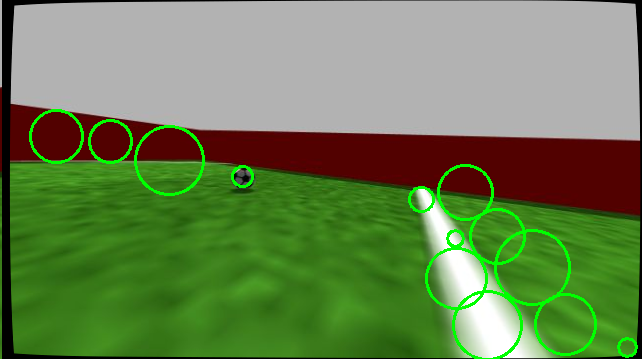
\includegraphics[width=7cm]{images/hough.png}
\centering
\caption{An example output of the circular Hough transform}
\end{figure}

\subsection{SVM Classifier}
\label{section: svm-implement}

The classifier uses the histogram of oriented gradients feature vector to decide whether a ball candidate should be rejected. The HOG descriptor uses the scikit-image implementation and uses a cell size of 8x8 pixels and a block size of 2x2 cells. All images are resized to 32x32 pixels as the SVM requires that every input vector must be the same size. A size of 32 pixels was chosen as ball candidate image usually smaller than this size meaning that no data is lost by resizing, while still being small enough to be able to compute quickly. These factors result in the feature vector having 288 dimensions.

Two datasets were collected for training the classifier; one in simulation and one on a real ball. Each dataset contains approximately 2000 negative samples and 200 positive samples. The positive samples are augmented by horizontal mirroring and rotations of -20\degree, -10\degree, 10\degree, 20\degree to increased the number of samples 10 times. Therefore there are also effectively 2000 positive samples, and the classifier is trained on approximately 4000 images. The datasets were collected by storing images of ball candidates that the system detected during the running of a basic ball chasing script. Each image was then manually labelled. 

Figure \ref{fig:comparing classifiers} shows the results of the comparison of various classifiers: k-nearest neighbours (k=5), k-nearest neighbours (k=15), linear SVM, SVM using the radial basis function (RBF) kernel, random forest and AdaBoost. Of these the SVM using the RBF kernel had the best results with a precision of 99.2\% and a recall of 96.1\% while having the second best classify time, only marginally slower than the linear SVM. Therefore the SVM with RBF kernel is the classifier used in the final implementation.

\begin{figure}[H]
    \centering
    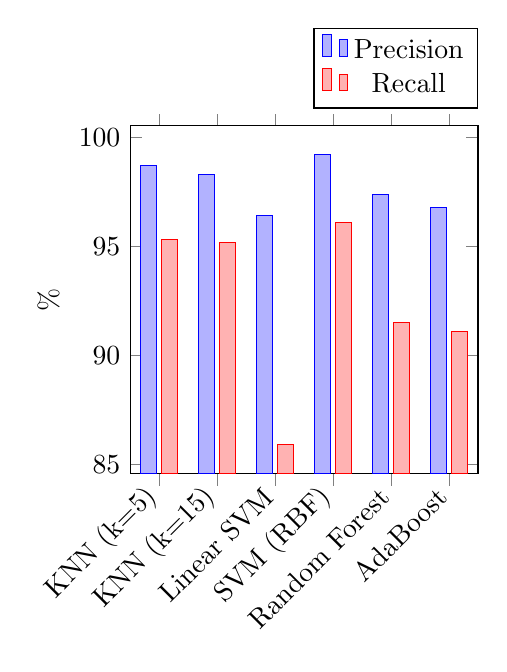
\begin{tikzpicture}
        \begin{axis} [ybar,
            height=6cm,
            width=6cm,
            bar width=0.2cm, 
            xlabel={}, 
            ylabel={\%},
            xtick={0,1,2,3,4,5},
            xticklabels={KNN (k=5), KNN (k=15), Linear SVM, SVM (RBF), Random Forest, AdaBoost},
            % xticklabels={Precision, Recall},
            xlabel style={yshift=-1cm},
            x tick label style={
                rotate=45,
                anchor=east,
            },
            legend style={
                anchor=south east,
                at={(1,1.05)}
                }
            ]
        \addplot coordinates {(1, 98.3) (0, 98.7) (2, 96.4) (3, 99.2) (4, 97.4) (5, 96.8)};
        \addplot coordinates {(1, 95.2) (0, 95.3) (2, 85.9) (3, 96.1) (4, 91.5) (5, 91.1)};
        
        % \addplot coordinates {(0, 98.3) (1, 95.2)};
        % \addplot coordinates {(0, 96.4) (1, 85.9)};
        % \addplot coordinates {(0, 99.2) (1, 96.1)};
        % \addplot coordinates {(0, 97.7) (1, 90.0)};
        % \addplot coordinates {(0, 96.8) (1, 91.1)};
        
        \legend {Precision, Recall};
        \end{axis}
    \end{tikzpicture}
    \hfill
    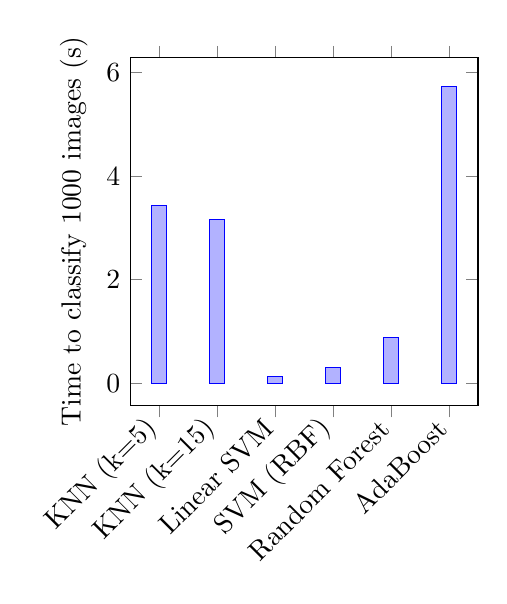
\begin{tikzpicture}
        \begin{axis} [ybar,
            height=6cm,
            width=6cm,
            bar width=0.2cm, 
            xlabel={}, 
            ylabel={Time to classify 1000 images (s)},
            xtick={0,1,2,3,4,5},
            xticklabels={KNN (k=5), KNN (k=15), Linear SVM, SVM (RBF), Random Forest, AdaBoost},
            xlabel style={yshift=-1cm},
            x tick label style={
                rotate=45,
                anchor=east,
            }
            ]
        \addplot coordinates {(1,3.163) (0, 3.43) (2,0.125) (3,0.299) (4,0.875) (5,5.729)};
        \end{axis}
    \end{tikzpicture}
    
    \caption{Comparing the performance of classifiers}
    \label{fig:comparing classifiers}
\end{figure}

\subsection{Image to World Space Conversion}
\label{section: image to world}

The MiRo Development Kit provides functions to convert a coordinate in image space and a range to a coordinate in world space. A view line is taken from the camera through the image space position, and a position can be found in head space by taking the position on the line corresponding to the range. The position in head space is then mapped into world space using the kinematic data of the MiRo. 

The range can be estimated by various methods. The first is to use a function mapping the radius of the ball in the image to a range, however this proved to be very noisy even when the ball is static. Another option is to obtain depth information from the image. Stereo depth is the obvious choice as the MiRo has stereo vision, however this limits the information to only the region shared by both cameras, and is time-consuming to tune to a reasonable accuracy. 

Instead of using the range to find the position on the view line, the final system uses the assumption that the ball is on the floor. This means that the z coordinate of the world position is already known to be at the center of the ball, or its radius so final coordinate can be calculated by finding the point at which the view line intercepts this height. 

This method results in more precise estimations, however there is a systematic error that can greatly decrease accuracy caused by imperfections in the camera calibration. The error can be corrected by applying offsets the azimuth and altitude of the view line according to the image space coordinates. 
The error in the azimuth correlates is fitted to a sine wave in the image x position and the altitude error is fitted to a polynomial regression in the image y position. As these corrections are specific to a camera calibration, they must be calculated independently for each MiRo. 

\subsubsection{Horizontal Coordinate System}

The horizontal coordinates system is a coordinate system that can be used to describe a 3-dimensional vector using 2 values. These values are the azimuth, which describes a rotation about the Z-axis or zenith and the altitude, which describes the rotation across the XY-plane.

\begin{figure}[H]
    \centering
    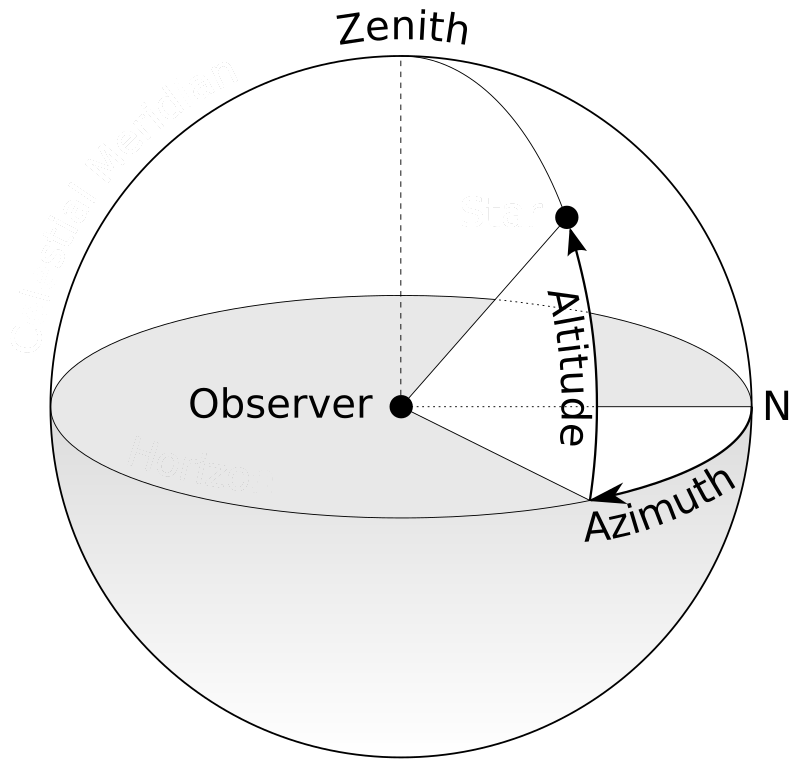
\includegraphics[width=7cm]{images/azal.png}
    \caption{Illustrating horizontal space coordinates}
    \label{fig:horizontal coordinates}
    Source: \url{https://en.wikipedia.org/wiki/Horizontal_coordinate_system} (edited)
\end{figure}
